\documentclass[a4,12pt]{article}
\usepackage{colortbl}
\usepackage{pgfplots}
\usepackage[margin=2cm]{geometry}
\pgfplotsset{compat=newest}
\begin{document}
\begin{table}
\footnotesize
\sffamily
\begin{center}
\begin{tabular}{cccccc}
Mean-Accuracy & \shortstack{clf1 \\ 0.5376} & \shortstack{clf3 \\ 0.5220} & \shortstack{clf2 \\ 0.5123} & \shortstack{clf4 \\ 0.4825} \\[1ex]
\shortstack{clf2 \\ 0.5123} & \cellcolor[rgb]{0.6355,0.7567,0.9983}\shortstack{\rule{0em}{3ex} -0.0253 \\ 60 / 0 / 68 \\ 0.5162} & \cellcolor[rgb]{0.7867,0.8448,0.9398}\shortstack{\rule{0em}{3ex} -0.0097 \\ 64 / 0 / 64 \\ 0.8102} & \cellcolor[rgb]{0.8674,0.8644,0.8626}\shortstack{\rule{0em}{3ex} Mean-Difference \\ r$>$c / r=c / r$<$c \\ Wilcoxon p-value} & \cellcolor[rgb]{0.9649,0.6402,0.5198}\shortstack{\rule{0em}{3ex} 0.0298 \\ 72 / 0 / 56 \\ 0.3880} \\[1ex]
\shortstack{clf4 \\ 0.4825} & \cellcolor[rgb]{0.3286,0.4397,0.8696}\shortstack{\rule{0em}{3ex} -0.0551 \\ 59 / 0 / 69 \\ 0.1018} & \cellcolor[rgb]{0.4839,0.622,0.9748}\shortstack{\rule{0em}{3ex} -0.0395 \\ 58 / 0 / 70 \\ 0.2835} & \cellcolor[rgb]{0.5869,0.7181,0.9989}\shortstack{\rule{0em}{3ex} -0.0298 \\ 56 / 0 / 72 \\ 0.3880} & \cellcolor[rgb]{0.8674,0.8644,0.8626}\shortstack{\rule{0em}{3ex} If in bold, then \\ p-value $<$ 0.05} \\[1ex]
\end{tabular}\\
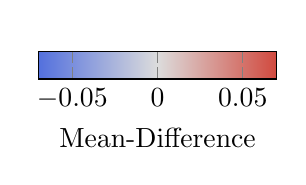
\begin{tikzpicture}[baseline=(current bounding box.center)]\begin{axis}[hide axis,scale only axis,width=0sp,height=0sp,colorbar horizontal,colorbar style={width=0.25\linewidth,colormap={cm}{rgb255(1)=(83,112,221) rgb255(2)=(220,220,220) rgb255(3)=(209,73,62)},colorbar horizontal,point meta min=-0.07,point meta max=0.07,colorbar/width=1.0em,scaled x ticks=false,xticklabel style={/pgf/number format/fixed,/pgf/number format/precision=3},xlabel={Mean-Difference},}] \addplot[draw=none] {0};\end{axis}\end{tikzpicture}\end{center}
\caption{[...] \textbf{If in bold, then p-value $<$ 0.05} [...]}
\end{table}
\end{document}
